\textbf{Глава 2} посвящена исследованию модельного порыва --- предельного решения на сепаратрисе, разделяющей в фазовом пространстве области притяжения решений, соответствующих ламинарному и турбулентному режимам течения. В предисловии к главе приведен краткий обзор работ, посвященных анализу решений на сепаратрисе в круглой трубе. 

В \textbf{разделе 2.1} описан метод получения модельного порыва. Предварительно найденное турбулентное решение $\v_{turb}(\x,t)$ используется в итерационной процедуре отыскания предельного решения на сепаратрисе. Задача решается с начальным условием
\begin{equation} \label{edge_init_eq}
\v(\x,t=0) = \v_{Pois}(\x)+\alpha(\v_{turb}(\x,t=t_0) - \v_{Pois}(\x)),
\end{equation}
где $\v_{Pois}=(1-r^2,0,0)$ --- течение Пуазейля, $t_0$ --- некоторый фиксированный момент времени, $\alpha$ --- скалярный параметр. Значение $\alpha=0$ соответствует нулевому возмущению и решением при $t > 0$ остается течение Пуазейля. При $\alpha=1$ уже в начальный момент времени реализуется турбулентный режим, который сохраняется при $t > 0$. При промежуточных значениях $\alpha$ происходит стремление решения либо к одному, либо к другому режиму. Применяя метод деления отрезка пополам, мы отыскиваем то значение $\alpha$, при котором решение эволюционирует на сепаратрисе, разделяющей области притяжения двух режимов течения. На Рисунке \ref{bisection_pic} представлены графики $A(t)$ – среднеквадратичного по всему объему отклонения поля скорости от течения Пуазейля для нескольких значений $\alpha$, демонстрирующие сходимость итерационного процесса. При уточнении значения $\alpha$ продлевается длительность балансирования решения на сепаратрисе.

\begin{figure}
\center{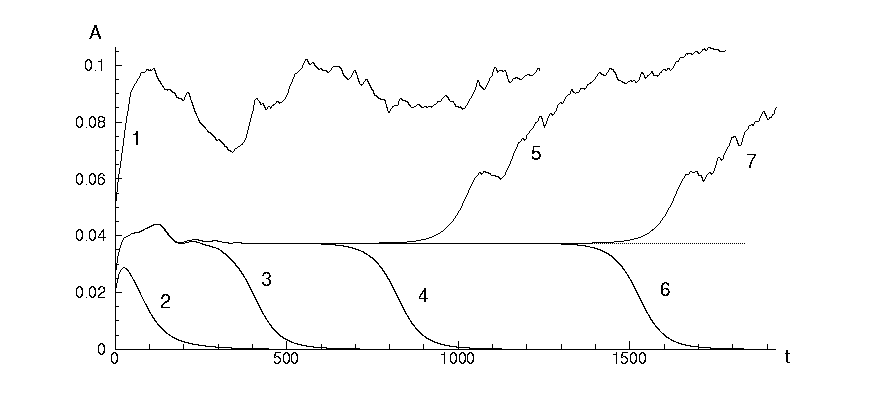
\includegraphics[width=1\linewidth]{bisection.png}}
\caption{Итерационный процесс построения решения на сепаратрисе}
\label{bisection_pic}
\end{figure}

В согласии с (Avila et al. 2013), при $\Re=2200$ и дополнительных условиях диаметральной симметричности и $\pi$-периодичности в угловом направлении решение на сепаратрисе постепенно выходит на условно периодический режим. Предельное решение на сепаратрисе описывает пространственно локализованную структуру длиной около $40R$, перемещающуюся вдоль трубы со скоростью $c=0.69U$. В сопутствующей системе отсчета поле скорости в каждой точке испытывает периодические колебания с периодом $T=60R/U$. 

Визуализация мгновенного поля скорости модельного порыва приведена на Рисунке \ref{edge_3D_img} (построена так же, как визуализация турбулентного порыва на Рисунке \ref{puff_3D_img}). Модельный порыв воспроизводит ряд характерных особенностей турбулентного порыва. В частности, модельный порыв имеет систему вытянутых вдоль стенки полос повышенной и пониженной скорости, но в этом случае полосы сохраняют свое положение в пространстве и испытывают лишь незначительные колебания около положения равновесия. 

\begin{figure}
\center{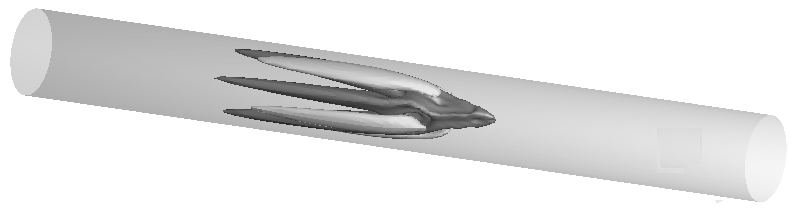
\includegraphics[width=0.9\linewidth]{edge_3D.png}}
\caption{Визуализация численного расчета модельного порыва}
\label{edge_3D_img}
\end{figure}

В \textbf{разделе 2.2} описаны основные свойства модельного порыва. В подвижной системе отсчета поле скорости модельного порыва $\v$ представляется в виде суперпозиции стационарной составляющей $\V = \overline{\v}^t$ и колебательной $\v_n = \v - \V$. Черта над выражением обозначает осреднение по указанной переменной. Стационарная составляющая, в свою очередь, представляется в виде суперпозиции осесимметричной $\V_{2D} = \overline{\V}^{\theta}$ и трехмерной $\V_{3D} = \V - \V_{2D}$ составляющих. 

В трехмерную стационарную составляющую движения $\V_{3D}$ попадают полосы повышенной и пониженной скорости. Изолинии $V_{x, 3D}$ в поперечном сечении трубы, в котором колебания имеют существенную амплитуду, изображены на Рисунке~\ref{mp_cs_pic}(a). В соответствии с наложенными условиями симметрии расчет проводится в одной четверти трубы. В каждом сечении трубы полосы пониженной скорости ($V_{x,3D} < 0$, прерывистые линии) проходят через центр расчетной области. Полосы повышенной скорости ($V_{x,3D} > 0$, сплошные линии) попадают на границы расчетной области в угловом направлении. 

\begin{figure}
\center{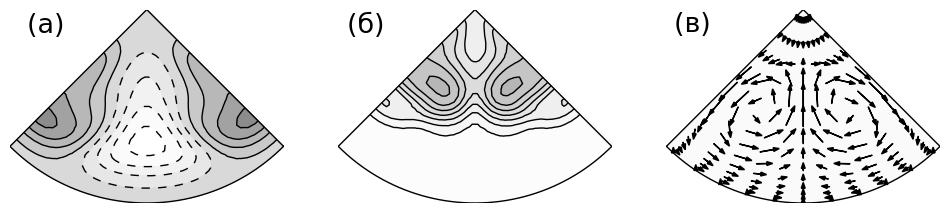
\includegraphics[width=1\linewidth]{mp_cs.png}}
\caption{Различные компоненты движения модельного порыва}
\label{mp_cs_pic}
\end{figure}

На Рисунке \ref{mp_cs_pic}(б) приведено распределение среднеквадратичной амплитуды пульсационной составляющей движения $\v_n$. Пульсации сконцентрированы между соседними полосами повышенной и пониженной скорости, а также между полосой ускорения и осью трубы. Пульсационная составляющая движения $\v_n$ напоминает бегущую вниз по порыву волну. Её фазовая скорость близка к $0.77U$, а длину можно оценить в $5R$. 

В \textbf{разделе 2.3} показано, что за образование полос повышенной и пониженной скорости ответственен лифтап (lift-up) эффект, связанный с движением жидкости в перпендикулярной к основному потоку плоскости. Векторное поле поперечной компоненты среднего течения $\V_{3D}$ приведено на Рисунке \ref{mp_cs_pic}(в). Оно соответствует наличию продольных вихрей, поддерживающих существование полос. Частицы жидкости, перемещающиеся от стенки в сторону оси трубы, приносят дефект скорости и образуют полосу замедления, а частицы, двигающиеся в противоположном направлении --- от оси к стенке, образуют полосу ускорения. Говорить о продольных вихрях позволяет также тот факт, что средняя продольная завихренность $\Omega_x$ оказывается сконцентрирована в небольших областях между соседними полосами повышенной и пониженной скорости. Распределение $\Omega^2_x$ по сечению трубы представлено на Рисунке \ref{OXgen_pic}(a).

\begin{figure}
\center{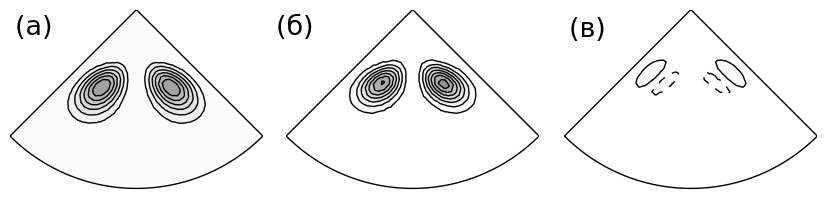
\includegraphics[width=1\linewidth]{autoref_OXgen.png}}
\caption{Механизм генерации продольных вихрей}
\label{OXgen_pic}
\end{figure}

В \textbf{разделе 2.4} показано, что пульсации возникают в результате линейной неустойчивости среднего течения. Для этого линеаризованные относительно возмущений уравнения с некоторыми случайными начальными условиями интегрировались по времени до выхода решения на режим экспоненциального изменения. Обнаружено, что $\V$ неустойчиво. Растущее возмущение $\v'_1 \sim e^{(\lambda+i\omega)t}$ имеет инкремент нарастания $\lambda=0.012$ и частоту $\omega=0.116$, близкую к частоте колебаний $2\pi/60=0.105$ в модельном порыве. Поле скорости растущего решения $\v'_1$ достаточно точно повторяет поле скорости пульсационной составляющей движения модельного порыва $\v_n$. 

В \textbf{разделе 2.5} рассматривается вопрос влияния продольной неоднородности среднего течения на форму пульсаций. Для этого на устойчивость исследованы однородные вдоль трубы поля скорости $\U_i = \V\big|_{x=x_i}$, повторяющее среднее течение в сечениях $x = x_i$ из области, в которой пульсации имеют существенную амплитуду. Показано, что продольная неоднородность среднего течения не является необходимым условием для возникновения пульсаций.

В \textbf{разделе 2.6} на основе уравнений движения анализируется вклад каждой из компонент движения в производство кинетической энергии других компонент движения. Это позволяет более строго обосновать полученные представления о взаимодействии между различными компонентами движения и показать, что все существенные взаимодействия учтены.

В \textbf{разделе 2.7} приведены выводы по главе. Основные результаты, приведенные в главе, опубликованы в работах автора диссертации \cite{MZG2015, Kazan2015, KMU2014, KMU2015}.


